\section{Theorie} 
\label{sec:Theorie}

In diesem Kapitel werden die theoretischen Hintergründe dieses Versuches erläutert. Dabei wird insbesondere auf die in der Durchführung verwendeten Schaltungen eingegangen.


\subsection{EM-Wellen}
\label{sec:themwellen}
Elektromagnetische Wellen, kurz EM-Wellen sind transversale Wellen. Sie schwingen also senkrecht zu ihrer
Ausbreitungsrichtung. Dabei steht das magnetische Feld immer senkrecht auf dem elektrischen Feld.
Im allgemeinsten Fall lassen sie sich durch folgende Gleichung beschreiben:
\begin{equation}
    \label{eq:wellenfunktion}
    A(x,t)=A_0sin(kx+\omega t+\phi_0)
\end{equation}
dabei ist $A_0$ die Amplitude, $k$ die Wellenzahl, $x$ der Ort, $\omega$ die Kreisfrequenz, $t$ der Zeitpunkt
und $\phi$ eine feste Phase weclche meist gleich null gesetzt wird. Eine solche Welle wird als laufend bezeichnet, bei positivem Vorzeichen der Kreisfrequenz
ist sie linkslaufend sonst rechtslaufend.


\subsubsection{Stehende Welle}
\label{sec:thstehendewelle}
Wenn eine laufende Welle senkrecht auf eine Grenzfläche trifft und dort totalreflektiert wird,
interferieren die einlaufende und die auslaufende Welle miteinander ud es entsteht eine Welle
mit scheinbar ortsfesten Knoten und Bäuchen. Eine solche Welle lässt sich mathematisch durch überlagerung
einer links- und einer rechtslaufenden Welle schreiben:
\begin{equation}
    \label{eq:stehendewelle}
    A(x,t)=A_0sin(xk+\omega t +\phi_0)+B_0sin(xk-\omega t +\phi_0)
\end{equation}
Dieser Ausdruck lässt sich für $A_0=B_0$ vereinfachen zu:
\begin{equation}
    A(x,t)=A_0sin(kx)cos(\omega t)
\end{equation}

\subsection{Stehwellenverhältnis}
\label{sec:thstehwelle}
In realen Systemen wird eine Welle nur selten totalreflektiert sondern meist nur teilreflektiert
und obendrein noch gestreut sodass die rücklaufende Welle gegenüber der hinlaufenden Welle eine
kleiner Amplitude hat. Nun muss also \autoref{eq:stehendewelle} verwndet werden. Da sich die Wellen 
jetzt nichtmehr vollständig auslöschen und auch die konstruktive Interferenz weniger wird, ergibt 
sich eine Welle welche zwischen zwei Niveaus von Feldstärken hin und herschwingt. Die Welle 
wird wieder zur laufenden Welle welche allerdings eine stehende Welle als Einhüllende hat.
An dieser stehenden Welle kann das sogenannte Stehwellenverhältnis gemessen werden. Es ist das 
Verhätnis zwischen der Feldstärke an einem Maximum un der an einem Minimum.
\begin{equation}
    \label{eq:stehwellenverhaeltnis}
    S=\frac{E_{max}}{E_{min}}
\end{equation}
Je näher mann der perfekten totalreflexion kommt desto mehr nähert sich S der eins an.
Das Stehwellenverhältnis wird in diesem Versuch auf zwei weisen ermittelt, zunächst mit der
später noch genauer erläuterten 3dB-Methode, hier ergibt es sich über:
\begin{equation}
    \label{eq:dreidB}
    S=\sqrt{1+\frac{1}{sin^2(\frac{\pi (x_{links}-x_{rechts})}{\lambda_H})}}
\end{equation}
Das kann unter der annahme das das Argument im Sinus ausreichend klein ist und der Bruch an sich 
dadurch so groß wird das die addierte 1 keine rolle mehr spielt mit der Kleinwinkelnäherung zu folgender
Formel vereinfacht werden:
\begin{equation}
    \label{eq:3dBleicht}
    S=\frac{\lambda_H}{(x_{links}-x_{rechts})}
\end{equation}
Im weiteren wird das Stehwellenverhältnis noch mit der ebenfalls später genauer erläuteten Abschwächer 
Methode ermittelt. Hier ergibt es sich über den Zusammenhang:
\begin{equation}
    S=10^{\frac{A_2-A_1}{20dB}}
\end{equation}

\subsection{Mikrowellen}
\label{sec:thallgemein}
Mikrowellen sind je nach definition Wellen mit Wellenlängen mit Wellenlängen von etlichen zentimetern bis
zu Bruchteilen von millimetern. Das entspricht Frequenzen von etwa 300 MHz bis 1 THz. In diesem Versuch werden
Wellen im bereich von wenigen GHz verwendet. Das entspricht Wellenlängen von wenigen zentimetern und hat den
Grund das für solche Wellenlängen passende Hohlleiter gut zu handhaben sind.

\subsection{Das Klystron}
\label{sec:thklystron}
Zur erzeugung der Mikrowellen kann ein Klystron verwendet werden. Ein Klystron besteht im allgemeinen 
aus zwei Hohlraumresonatoren und einer dazwischen gelegenen Driftstrecke. In den ersten Hohlraumresonator 
wird ein Schwingung mit passender Frequenz eingekoppelt, dann wird ein Elektronenstrahl eingeführt, welcher 
von der Schwingung im Resonator Moduliert wird. Das heißt Teilchen werden, da das elektrische Feld ortsabhängig
ist, ortsabhängig beschleunigt oder abgebremst. So bilden sich über die Driftstracke 
einzelne Elektronenpakete die Bunches genannt werden. Diese Bunches erzeugen im zweiten Hohlraumresonator eine
zur im ersten Resonator eingekoppelten Schwingung, bedeutend stärkere Schwingung. Hiervon kann ein kleiner Teil 
ausgekoppelt werden und für das Experiment vervendet werden. In deiesem Versuch wird jedoch kein klassisches
Klystron sondern das sogenannte Reflexklystron verwendet. Die besonderheit ist hier das es nur einen Resonator 
gibt in welchem die Schwingung sowohl ein als auch ausgekoppelt wird. Dazu wird der Elektronenstrahl am Ender der 
Driftstrecke von einer Kathode reflektiert und wieder in den Resonator geleitet wo dann wieder eine Schwingung
erzeugt wird. Optimale verstärkungen werden erzeugt wenn die ein und augekoppelte Welle Phasengleich sind. 
Die Phasenverschiebung lässt sich über die länge der Driftstrecke steuern. Die Länge der Driftstrecke kann 
sowohl durch mechanische verschiebung der reflektierenden Kathode als auch durch ihre Spannung gegenüber 
der Anode verändert und eingestellt werden. Die optimalen Verstärkungen liegen bei Transitzeiten von
$\tau=T_0(n+\frac{3}{4})$ mit $n \in \mathbb{N}$ und $T_0$ der Periodendauer der eingekoppelten Schwingung.

\begin{figure}
    \centering
    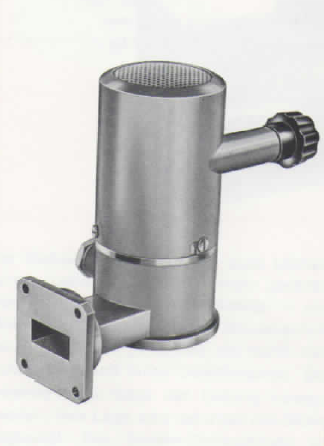
\includegraphics[width=0.3\textwidth,angle=0]{content/grafiken/Klystron.PNG}
    \caption{Das benutzte Reflexklystron PM 7011 X [1]}
    \label{fig:Klystron}
  \end{figure}

\subsection{Der Hohlleiter}
\label{sec:thwellenleiter}
Ein Hohlleiter für Elektromagnetische Wellen ist im allgemeinen ein Rohr aus einem Material welches in der 
Lage ist elektrischen Strom zu leiten. Er dient dazu Energie in Form von EM-Wellen gebündelt zu leiten und
eine Ausbreitung in alle Raumrichtungen einzuschränken. Der Querschnitt eines Hohlleiters ist im Grunde 
beliebig. In der Praxis werden jedoch aufgrund der vergleichsweise einfachen berechenbarkeit meist rechteckige
runde oder allenfalls ovale Querschnitte gewählt. In diesem Versuch werden Hohlleiter mit einem rechteckigen
Querschnitt verwendet. Jeder Hohlleiter hat eine sogenannte Cutoff Wellenlänge $\lambda_c$ das ist die maximale
Wellenlänge also minimale Frequenz welche die eingekoppelte Welle haben darf um noch übertragen zu werden.
Sie ist bei der rechteckigen Variante abhängig von der Breite $a$ des Hohlleiters, $\lambda_c=2a$ an diesem Punkt
passt genau noch eine Halbwelle zwischen die Seitenwände des Hohlleiters. Im Hohlleiter können sich zwei verschiedene
Grundmoden ausbreiten, einerseits die "transversal elektrische" TE-Mode bei der das elektrische Feld eine Komponente
in Ausbreitungsrichtung auweist und andererseits die "transversal magnetische" TM-Mode bei welcher das Magnetfeld
eine Komponente in Ausbreitungsrichtung aufweist. Die Wellen werden mit $H_{nm}$ bzw. $E_{nm}$
bezeichnet. n steht hier für die Anzahl der Wellenmaxima in horizontaler Richtung während m für die Anzahl der 
Wellenmaxima in Vertikaler Richtung steht. Jeder Hohlleiter hat einen charakeristischen frequenzabhängigen
Wiederstand der Impedanz genannt wird. Er kommt duch den Ohmschen Wiederstand des Materials des Hohlleiters
und durch Inperfektionen der Oberflächen, an welchen die Wellen gestreut werden, zustande.

\begin{figure}
    \centering
    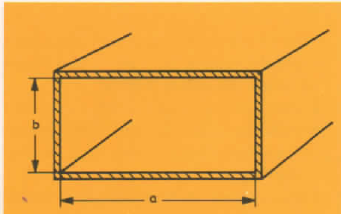
\includegraphics[width=0.3\textwidth,angle=0]{content/grafiken/Hohlleiter.PNG}
    \caption{Zeichnung des benutzten Hohlleiters. [1]}
    \label{fig:Hohlleiter}
  \end{figure}

